\chapter{Metodología Empleada}
\label{sec:metodologia}

\section{Instrumental de Medición y Registro}
Para el relevamiento sonoro se utilizó un dispositivo móvil Android equipado con la aplicación \textit{Sound Analyzer v2.7},
configurada como sonómetro integrador de Clase 2 conforme a la norma IRAM 4074. El instrumento cuenta con certificación de
calibración acústica previa realizada el 14 de agosto de 2026. Los parámetros de configuración del ensayo fueron:
\begin{itemize}[noitemsep]
  \item Ponderación frecuencial: Filtro A ($\dBA$).
  \item Ponderación temporal: Rápida (Fast, $F = 125\ms$).
  \item Parámetros registrados: $L_{AF}$, $L_{Aeq}$.
  \item Frecuencia de muestreo continuo: Muestreo segundo a segundo ($t_{total} = 306,69\s$).
\end{itemize}

\section{Descripción del Puesto de Trabajo y Tarea Simulada}
El ensayo se realizó en un banco de trabajo para reparación de electrodomésticos (Figura~\ref{fig.ej1:puesto_trabajo}).
El puesto consta de una mesa de apoyo de granito sobre la cual se disponen los componentes de un electrodoméstico en
desarme (motor eléctrico, polea de transmisión, correa y tornillería) y la herramienta de mano.

\begin{figure}[!ht]
  \centering
  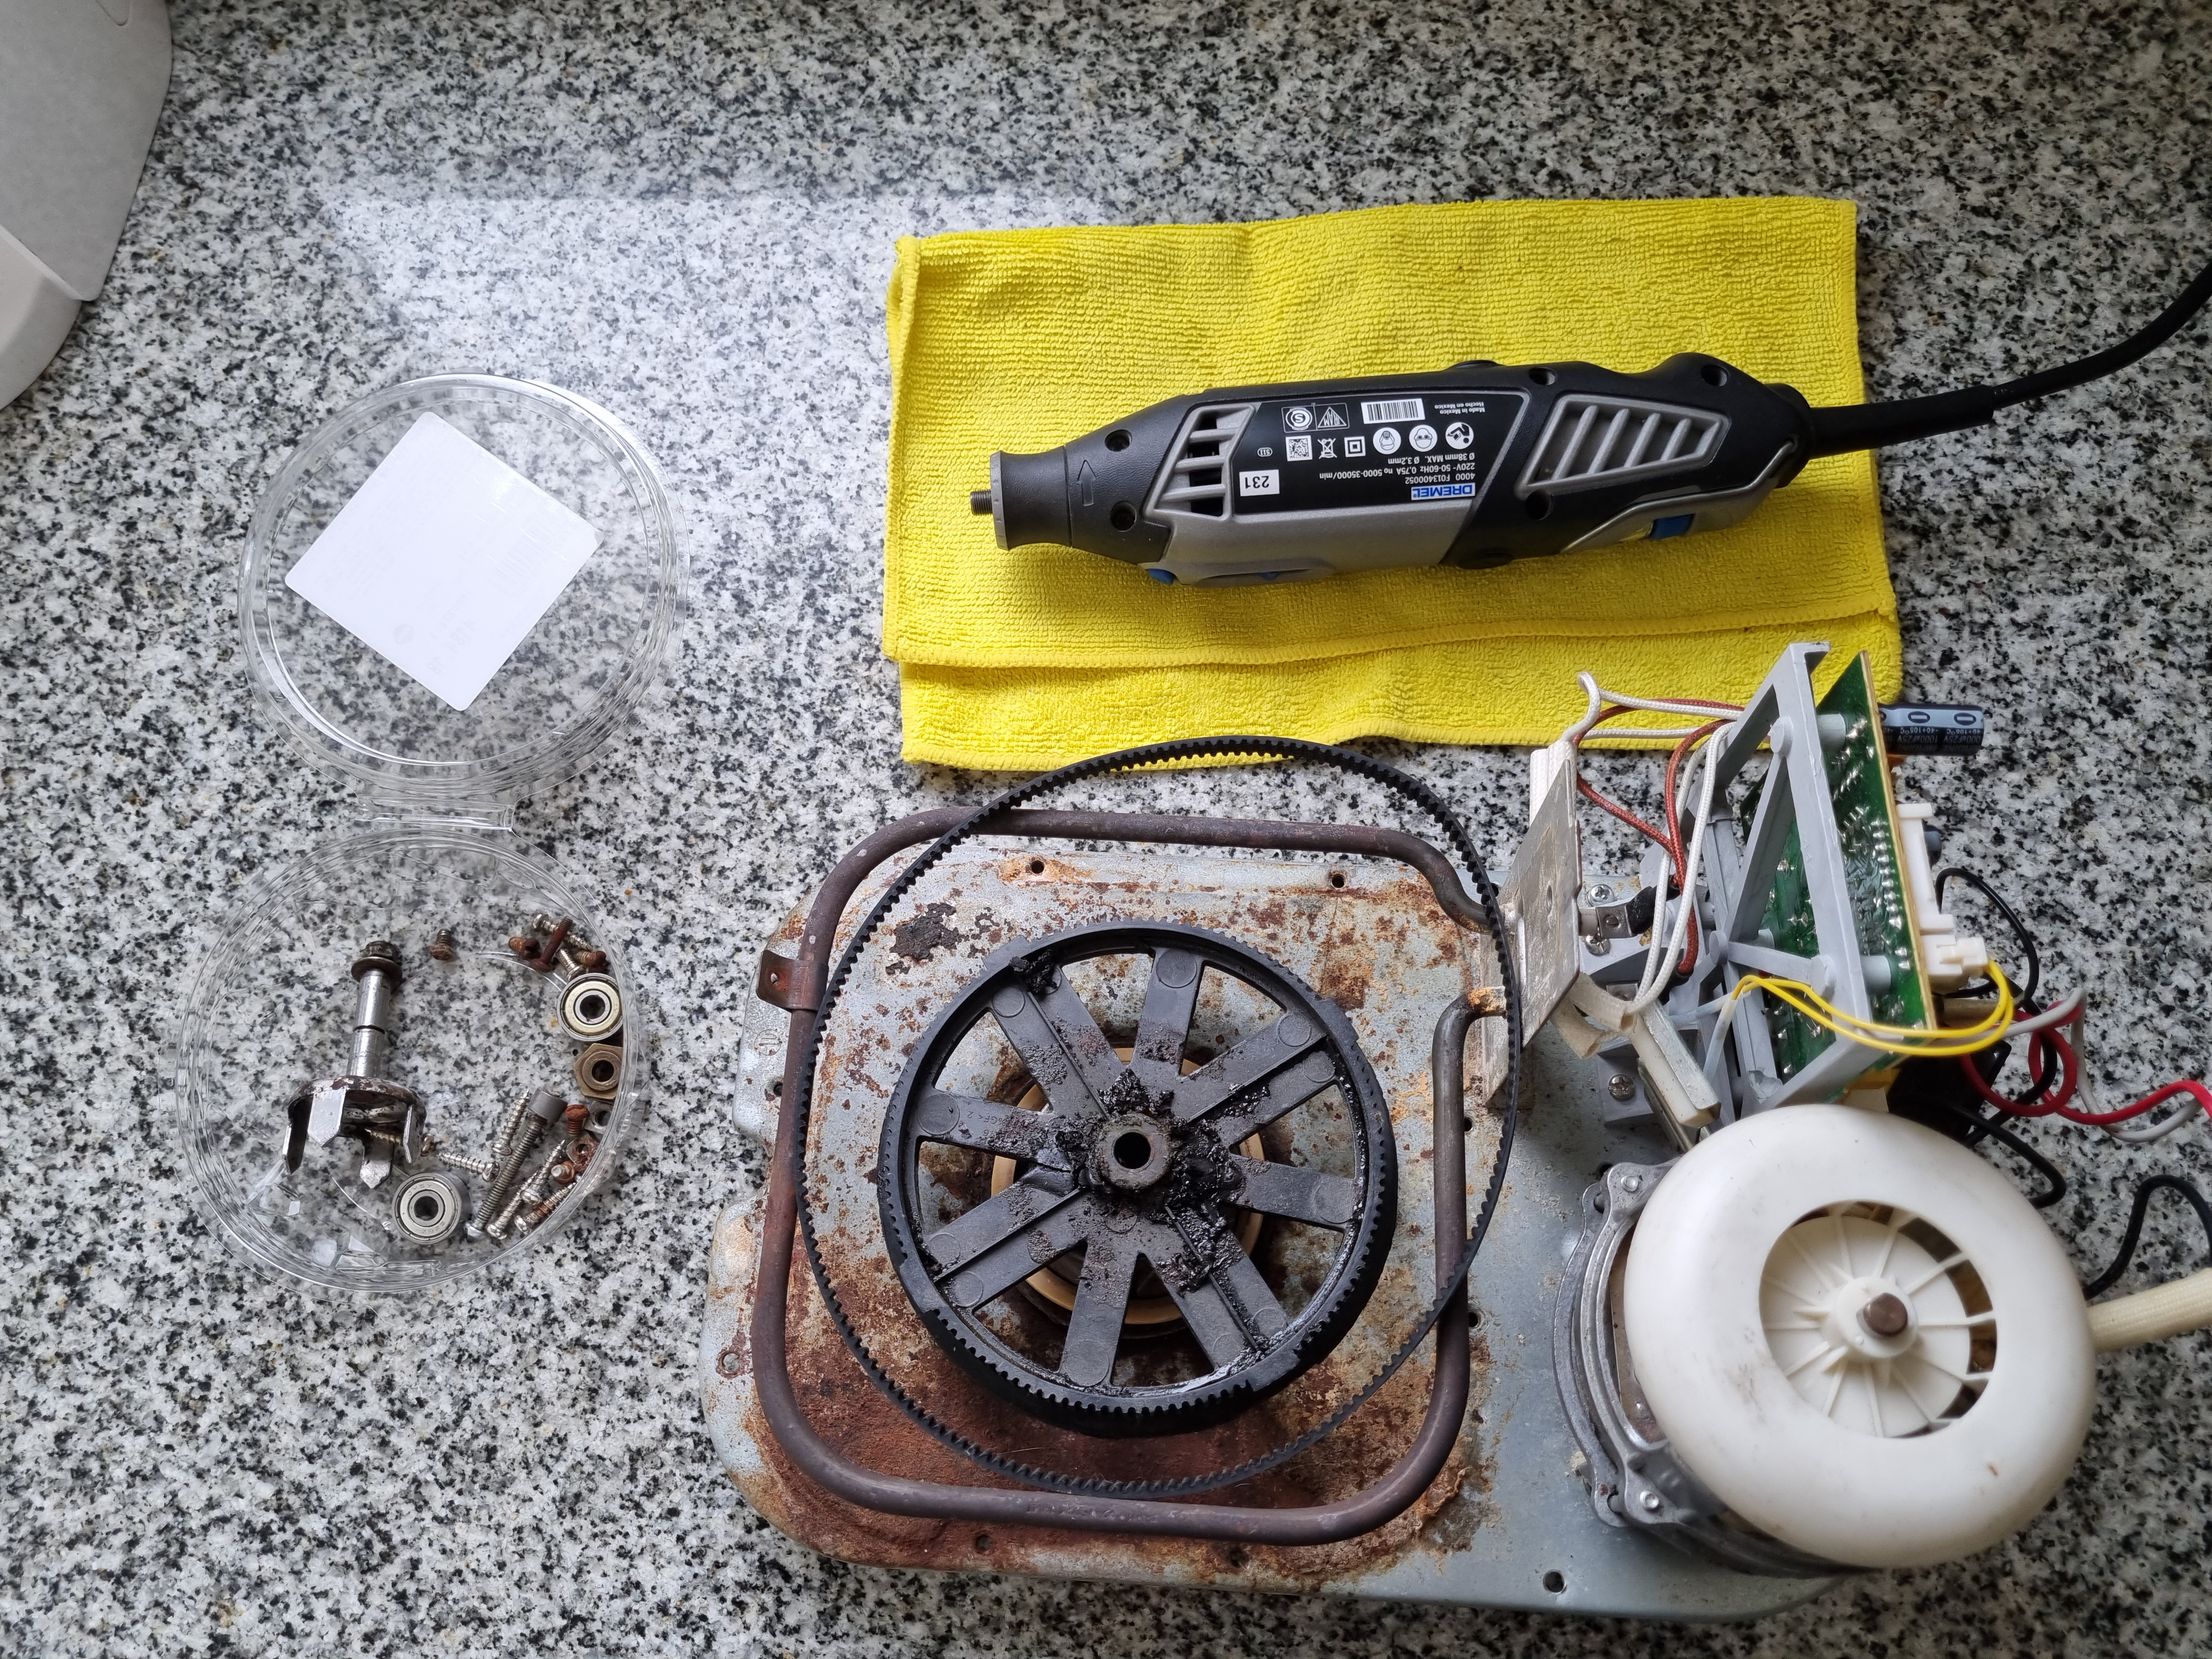
\includegraphics[width=0.75\textwidth]{pictures/puesto_dremel.jpg}
  \caption{Puesto de trabajo simulado de reparación de electrodomésticos y minitorno Dremel.}
  \label{fig.ej1:puesto_trabajo}
\end{figure}

La herramienta evaluada es un minitorno \textit{Dremel} de alta velocidad. El patrón operativo del trabajador se estructuró
según un régimen intermitente compuesto por ciclos repetitivos de $30\s$ de trabajo activo y $5\s$ de reposicionamiento.
El ensayo de $300\s$ se dividió en dos etapas bien definidas:
\begin{enumerate}
  \item \textbf{Etapa 1 ($0\s$ a $150\s$):} Operación del minitorno a $15.000\text{ RPM}$, simulando tareas
        de corte de tornillos agarrotados y ajuste de piezas metálicas.
  \item \textbf{Etapa 2 ($150\s$ a $300\s$):} Operación del minitorno a $25.000\text{ RPM}$, simulando tareas
        de pulido, rectificado y desoxidado de ejes con accesorio de cepillo rotativo.
\end{enumerate}

\section{Disposición del Sensor y Condición de Ensayo}
El sensor de captación acústica se ubicó a la altura del oído del operario ($1,50\m$ respecto al suelo) y a una distancia
de $0,50\m$ de la zona de contacto entre la herramienta y la pieza de trabajo, garantizando la representatividad del campo
sonoro en la zona auditiva durante los $306,69\s$ de ensayo ininterrumpido.
